\documentclass[10pt,a4paper]{article}
\usepackage[utf8]{inputenc} % para poder usar tildes en archivos UTF-8
\usepackage[spanish]{babel} % para que comandos como \today den el resultado en castellano
\usepackage{a4wide} % márgenes un poco más anchos que lo usual
\usepackage[conEntregas]{caratula2}
\usepackage{float}
\usepackage[pdftex]{graphicx}
\usepackage{caption}
\usepackage{subcaption}
\usepackage{amsmath,amssymb}
\usepackage{algorithm}
\usepackage{algpseudocode}
\usepackage{pifont}

%Esto de abajo es para encabezado y pie de pagina
\usepackage{lastpage}
\usepackage{fancyhdr}
\usepackage{ulem}
% Simbolos matemáticos
%\usepackage{amsmath}
%\usepackage{amsfonts}
%\usepackage{amssymb}
%\usepackage{algorithm}
%\usepackage{algpseudocode}
% Descoración y gráficos
%\usepackage{fancyhdr}
%\usepackage{multirow}
%\usepackage{alltt}
\usepackage{listings}
\usepackage{color}

\definecolor{mygreen}{rgb}{0,0.6,0}
\definecolor{mygray}{rgb}{0.5,0.5,0.5}
\definecolor{mymauve}{rgb}{0.58,0,0.82}

\lstset{ %
  backgroundcolor=\color{white},   % choose the background color; you must add \usepackage{color} or \usepackage{xcolor}
  basicstyle=\footnotesize,        % the size of the fonts that are used for the code
  breakatwhitespace=false,         % sets if automatic breaks should only happen at whitespace
  breaklines=true,                 % sets automatic line breaking
  frame=single,                    % adds a frame around the code
  keepspaces=true,                 % keeps spaces in text, useful for keeping indentation of code (possibly needs columns=flexible)
  keywordstyle=\color{blue},       % keyword style
  language=SQL,                 % the language of the code
  numbers=left,                    % where to put the line-numbers; possible values are (none, left, right)
  numbersep=5pt,                   % how far the line-numbers are from the code
  numberstyle=\tiny\color{mygray}, % the style that is used for the line-numbers
  rulecolor=\color{black},         % if not set, the frame-color may be changed on line-breaks within not-black text (e.g. comments (green here))
  showspaces=false,                % show spaces everywhere adding particular underscores; it overrides 'showstringspaces'
  showstringspaces=false,          % underline spaces within strings only
  showtabs=false,                  % show tabs within strings adding particular underscores
  stepnumber=1,                    % the step between two line-numbers. If it's 1, each line will be numbered
  stringstyle=\color{mymauve},     % string literal style
  tabsize=4,                       % sets default tabsize to 2 spaces
  title=\lstname                   % show the filename of files included with \lstinputlisting; also try caption instead of title
}

\pagestyle{fancy}

\cfoot{\thepage /\pageref{LastPage} }



\newcommand\BlockIf[1]{\KwSty{If} \\ #1 \\ \KwSty{End If}}
\newcommand\BlockElseIf[1]{\KwSty{Else If} \\ #1 \\ \KwSty{End Else If}}
\newcommand\BlockElse[1]{\KwSty{Else} \\ #1 \\ \KwSty{End Else}}

\begin{document}

\titulo{Trabajo Práctico}
\subtitulo{Sudoku}

\fecha{\today}

\materia{Metaheurísticas}
\submateria{2do Cuatrimestre de 2015}
%\grupo{Grupo 5}

\integrante{Kujawski, Kevin}{459/10}{kevinkuja@gmail.com}
\integrante{Ortiz de Zarate, Juan Manuel}{45/10}{jmanuoz@gmail.com}

% Pongan cuantos integrantes quieran

\maketitle

\newpage
\tableofcontents
%compilar varias veces si no se actualiza el indice o el pie de pagina

\newpage
\section{Introducción}
Sudoku es un juego de lógica cuyo objetivo es rellenar una cuadricula de tamaño 9x9, divididas a su vez en 9 cajas de 3x3, estas últimas llamadas cajas. Inicialmente contiene cierta cantidad de celdas con valores fijos pre-definidos y válidos, es decir, sus valores están entre [1,9], no hay repetidos por filas, columnas o cajas. \\Las reglas del juego son:
\begin{enumerate}
  \item Cada fila debe contener todos los números en el intervalo [1,9]
  \item Cada columna debe contener todos los números en el intervalo [1,9]
  \item Cada caja debe contener todos los números en el intervalo [1,9]
\end{enumerate}

El objetivo del juego es rellenar las celdas en blanco de la cuadricula inicial respetando las reglas del juego. A pesar de las simpleza del objetivo y las reglas del juego, hay 6670903752021072936960 formas posibles de ser rellenada una cuadricula. Buscar una solución intentando todas las formas posibles es claramente imposible, y eso incentiva la utilización de una metaheurística para solucionar el juego.\\
En el presente trabajo, presentaremos una posible formulación matemática del Sudoku como un problema de optimización e dos propuestas de implementación utilizando dos metaheurísticas: Simulated annealing y Colonia de hormigas

\section{Descripción y formulación matemática}


Nuestra formulación matemática es una adaptación de (2). En esa formulación, las variables $X_{ijk} $ son variables de decisión, definidas de la siguiente manera:
\[
X_{ijk}= \left\{ \begin{array}{lcc}
             1 &   $si el elemento (i,j) de la cuadricula contiene  el valor k$\\
             \\ 0 &  $en caso contrario$
             \end{array}
   \right.
   \]

   
  La formulación como programación lineal entera es la siguiente:	
\begin{equation*}
\begin{array}{ll@{}ll}
\text{min}  & \displaystyle $FuncionCosto(X)$ &\\
\text{sujeto a} & \displaystyle\sum\limits_{i=1}^{9} X_{ijk}=1, j=1:9,k=1:9 & (1)\\
		& \displaystyle\sum\limits_{j=1}^{9} X_{ijk}=1,i=1:9,k=1:9 & (2)\\
		& \displaystyle\sum\limits_{j=3q-2}^{3q} \sum\limits_{i=3p-2}^{3p} X_{ijk}=1, k=1:9,p=1:3,q=1:3 & (3) \\
                 & \displaystyle\sum\limits_{k=1}^{9} X_{ijk}=1, i=1:9,j=1:9 & (4)\\
                 & X_{ijk}=1 \forall (i,j,k) \in INICIALES &(5) \\
                 &  X_{ijk} \in {0,1}
\end{array}
\end{equation*}

 
 Hay que notar que como se trata de un problema de satisfacibilidad, la formulación no necesita de una función objetivo, por eso la definimos como 0. Las restricciones (1),(2) y (3) garantizan que cada numero en el intervalo posible de la instancia solo aparezca una vez en cada columna, fila, y caja, respectivamente. La restricción (4) garantiza que todas las posiciones de la martiz esten rellenas. La restricción (5) fuerza que las variables fijas de la instancia permanezcas sin alterar.


\newpage
\subsection{Hormigas}

En un principio intentamos resolver este problema con la metaheurística colonia de hormigas. Pero los resultados que obteníamos no eran buenos. Visto esto optamos por hacer algunos cambios en el algoritmo original para ver si podíamos optimizar las soluciones. Efectivamente logramos mejorar, a esta nueva metaheurística la llamamos Hormigas. Por el hecho de que las hormigas no salen en grupo sino individualmente. A continuación explicamos como qued\'o el proceso con nuestros cambios.
\paragraph{Clase Hormigas}
\begin{algorithmic}[1]
\Function{resolver}{Inicio }

\State $feromonas$ $\gets$ new Feromonas()
\For {1 to 400}
	\State $sudoku$ = new Sudoku()
	\State $hormiga$ = new Hormiga(sudoku,feromonas, probaSeguiFeromona)
	\If{la iteración es multiplo de 6}   
		\State{ feromonas$\to$evaporar() }
	\EndIf
	\If{hormiga$\to$resolver()}   
		\State{ devolver true }
	\EndIf
	
\EndFor

\State Devolver false
\EndFunction
\end{algorithmic}
\paragraph{Clase Hormiga}
\begin{algorithmic}[1]

\Function{resolver}{ }

\State casillas = $sudoku$ $\to$ obtenerCasillasSinValor()
\Comment Obtengo las casillas que aun no tienen valor seteado ordenadas por cantidad de valores posibles a insertar
\While {casilla = casillas$\to$obtener}
	\State $seMovio$ = seguirFeromona(casilla)	
	\If{no seMovio}   
		\State{ $seMovio$ = elegirRandom() }
		\If{no seMovio}   
			\State{ Devolver false }
			\Comment si no se movio quiere decir que no era posible insertar ningún valor, por lo tanto este camino no tiene soluci\'on
		\EndIf
	\EndIf
	\State casillas = $sudoku$ $\to$ obtenerCasillasSinValor()
	\Comment Vuelvo a obtener las casillas, porque si inserte un valor cambian los posibles de las muchas casillas
\EndWhile
\State{ Devolver true }
\Comment Si pude insertar valores en todas las que estaban vacias, entonces resolvi el sudoku
\EndFunction
\\
\Function{seguirFeromona}{casilla }
	\State valoresConFeromonas = feromonas$\to$ obtenerFeromonas(casilla)
	\Comment obtengo cada valor posible para esa casilla y cuanta feromona hay depositada en cada uno
	\While {valor = valoresConFeromonas$\to$obtener}
		\State probaMoverse = random(0,probaSeguiFeromona)
		\If( (valor$\to$feromona $\ast$ probaMoverse) $\>$ 100)
			\State moverse(casilla,valor)
			\State eliminarUltimaFeromonaDepostada() \Comment elimino la ultima feromona depositada porque seguro el ultimo valor insertado era incorrecto
			\State{ Devolver true }
		\EndIf
	\EndWhile
	\State{ Devolver false }
\EndFunction
\\
\Function{elegirRandom}{casilla }
	\State posiblesValores$\to$obtenerPosiblesValores()
	\If{posiblesValores no es vacio}   
		\State valor = posiblesValores$\to$elegirAlAzar()	
		\State moverse(casilla,valor)
		\State{ Devolver true }
	\EndIf
	\State{ Devolver false }
\EndFunction
\\
\Function{moverse}{casilla,valo }
	\State feromonas$\to$depositarFeromona(casilla,valor)
	\State sudoku$\to$insertarValor(casilla,valor)
\EndFunction
\end{algorithmic}


Coloquialmente lo que hace este algoritmo es, dado un sudoku incial lanzar 400 hormigas a intentar resolverlo. Cada una recorre las casillas vacias, comenzado por las que menos posibiles valores a insertar tienen (seg\'un las reglas del sudoku antes mencionadas). Para cada casilla se fija si alguno de los valores posibles tienen feromonas depositadas y en base a un calculo probabilistico inserta ese valor o no. Si no, elige uno de los posibles valores al azar y deposita una feromona en el mismo. Depositar una feromona consiste en incrementar en una unidad la probabilidad de que en esa casilla se elija ese valor.
\\
\\
Cada hormiga intenta solucionar el sudoku inicial pero utilizando las feromonas insertadas por sus predecesoras. Cada 6 hormigas, se produce la evapotaci\'on de las feromonas, este proceso consiste en restarle una unidad a cada valor de cada casilla (excepto que el mismo sea 0). Decidimos que sea cada 6 porque probando distintos sudokus vimos que aumentar este n\'umero mejoraba algunas soluciones pero empeoraba otras y lo mismo sucedía la inversa, 6 era el punto intermedio.
\\
\\
Son 400 porque probando varias veces el algoritmo y viendo que numero de hormiga es la que solucionaba el sudoku el mayor numero obtenido fué 350, por lo tanto 400 nos pareció una buena cota que no limite el llegar a la solución y a la vez tampoco aumente el computo innecesariamente.
\\
\\
Por \'ultimo el valor ``probaSeguiFeromona'' utilizado fué 2 porque tambi\'en en base a las pruebas realizadas fue el que mejor equilibrio establec\'ia para llegar a las soluciones en disintos sudokus (entre 1 y 8 variaba su efectividad entre los sudokus, a partir de este valor directamente no llegaba nunca a una soluci\'on)


\newpage
\section{Experimentos}

En primera instancia realizamos experimentos con ambas metaheurísticas a sudokus de distintos niveles de dificultad [3] y randoms (estos son sudokus solucionados a los que les blanqueamos de manera random 30 casillas). El objetivo es comparar los algoritmos entre sí para ver cuan efectivos son.


\begin{table}[ht]
\centering
\begin{tabular}{|l|l|l|}
\hline
          & \textbf{Simulated Annealing} & \textbf{Colonia de Hormigas} \\ \hline
{Escenarios probados} &       115                       &        115                      \\ \hline
{Total Solucionados} &                      70 (60\%)      &              60 (52\%)               \\ \hline
{Dificultad baja} &                     71 \%         &              69\%                \\ \hline
{Dificultad moderada} &                  40 \%            &             25 \%                 \\ \hline
{Dificultad alta} &                         16\%     &            5 \%                  \\ \hline
{Random} &                         63\%     &            60 \%                  \\ \hline
\end{tabular}
\end{table}



\subsection{Simulate annealing}
Para los experimentos elegimos un factor de enfriamiento en 0.5 y una temperatura inicial de 1. La justificación es en base a los experimientos realizados y que mostraremos en esta sección. \\ \\

El siguiente grafico es el resultado del tiempo que toma solucionar un Sudoku en donde partiendo de una solución existente blanqueamos celdas random y observamos como lo soluciona el algoritmo:\\
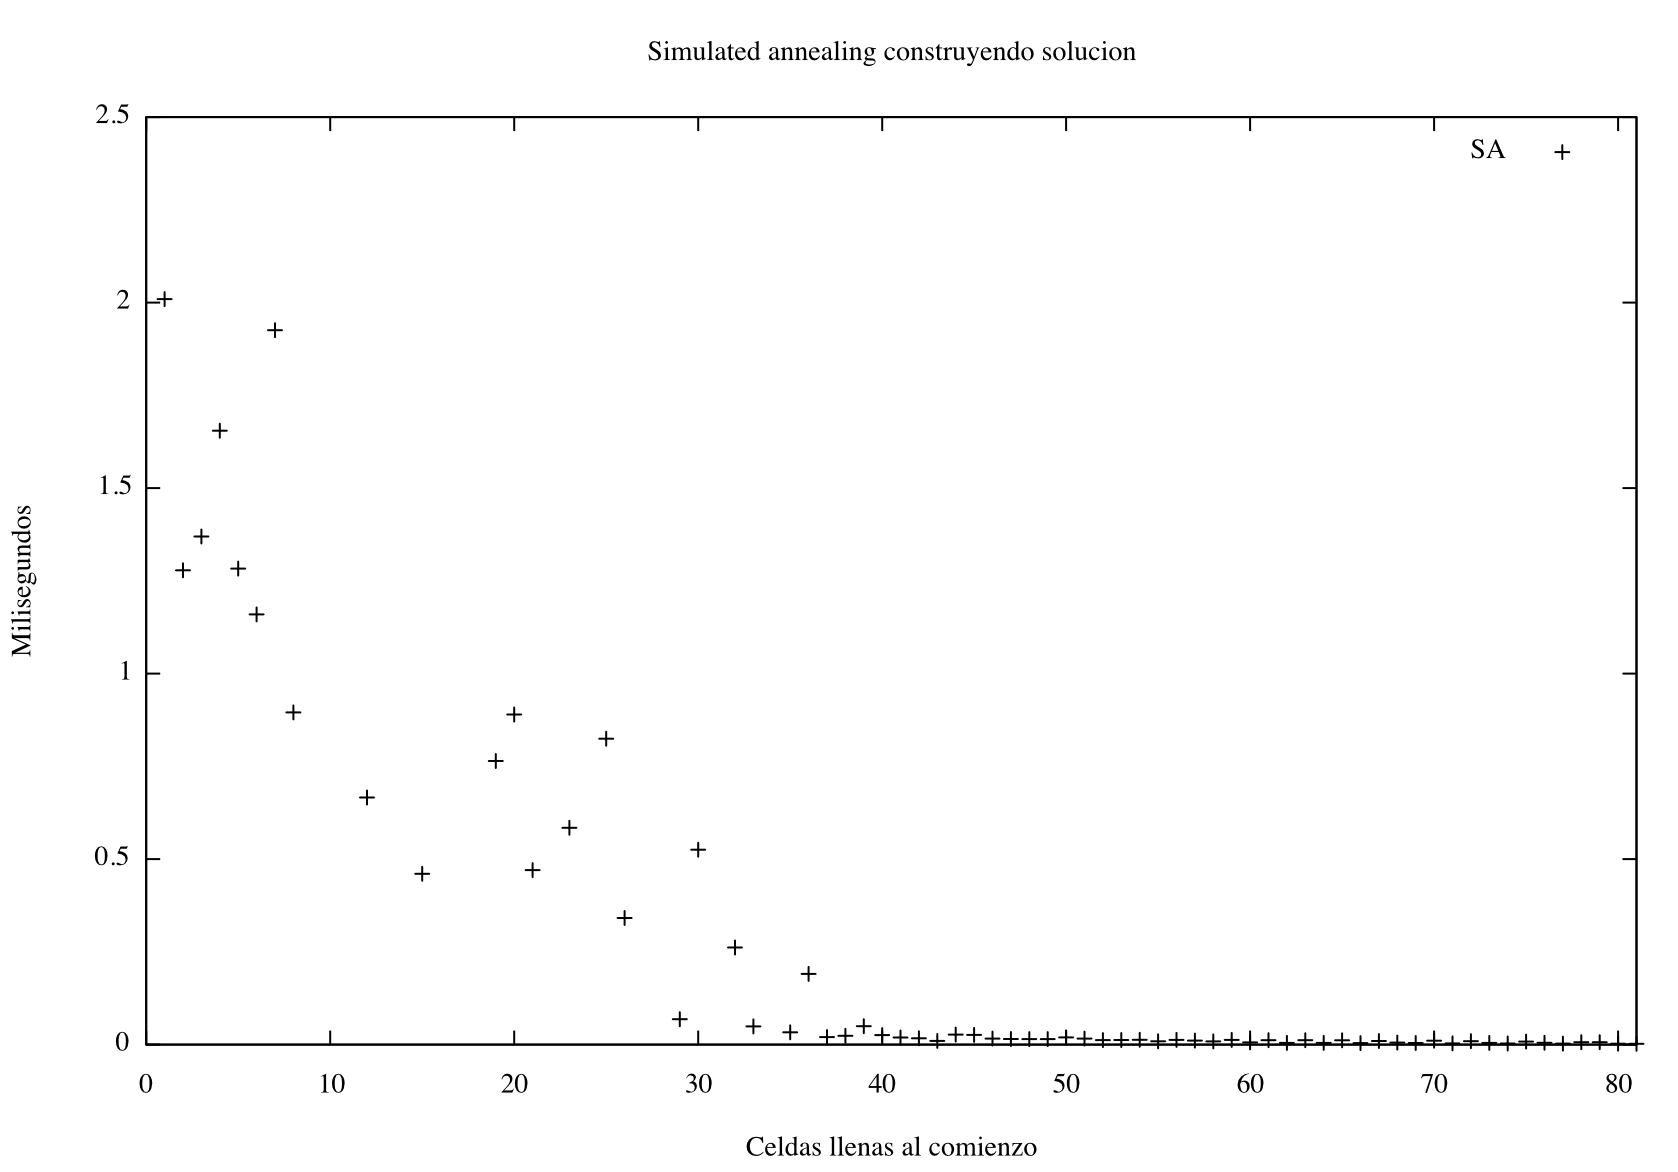
\includegraphics[scale=0.5]{imgs/randomSA.png}	\\
Clarmente se puede observar que a medida que el tablero esta mas lleno el tiempo es menor, eso es debido a la suma de varios factores, como que inicialmente infiere más celdas, son menos las vacias (que se convierte en menos iteraciones) y menos búsqueda de soluciones vecinas.\\\\

A continuación corrimos el algoritmo con 25 soluciones de diferentes niveles de dificultad, variando el factor de enfriamiento (o alfa):\\
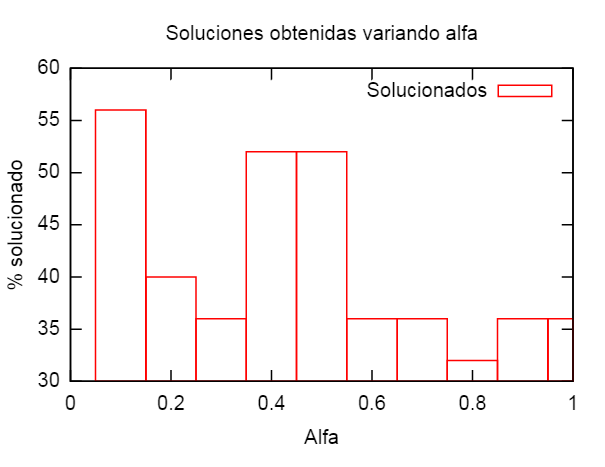
\includegraphics[scale=0.7]{imgs/porc_soluc.png}	\\
Si bien con valores intermedios (aprox 0.5) es donde se concentran las mejores soluciones, y que la mayor cantidad se logra con un 0.1, creemos en base a anteriores pruebas que el el factor de enfriamiento debería ser siempre mayor de 0.5 para que sea algo "lento" y no siempre elija ir por soluciones vecinas pero que tampoco las restrinja totalmente. 


\newpage
\section{Conclusiones}

En este trabajo, hemos presentado, a nuestro entender, dos aplicaciones de metaheurísticas para resolver el popular rompecabezas de 9x9 conocido como \textbf{Sudoku}. Hemos aplicado los algoritmos a distintos problemas tomados de sitios (de distintos grados de "dificultad"), y hemos visto en todas nuestras pruebas de que los algoritmos no llegan a conseguir cierta optimalidad (como suele ser el caso de las técnicas de optimización), logrando mejores resultados con el Simulated annealing respecto a la Colonia de Hormigas, pero consistentemente encuentran la solución en un tiempo razonable, ya que estamos hablando de un problema NP Completo. Para tener éxito, no depende necesariamente de casos problemáticos sino de la logica que se aplica en encontrar la solución (y de las distintas técnias propias del Sudoku que se puedan aplicar).\\
También es destacable que para los casos que no se puede llegar a una solución ideal, el costo o $"celdas ilegales"$ que se obtienen son bastante bajas, en el orden de las 2 a 5 y que muchas veces no dependen de los parámetros de entrada variables sino de la aleatoreidad de los algoritmos. \\
Creemos que a la hora de elegir entre las dos metaherísticas nos quedaríamos con Simulated annealing, ya que no solo obtuvimos mejores resultados sino que ademas \\
Por último, aunque hemos demostrado en este informe que este tipo de enfoque de búsqueda estocástico es capaz de resolver una gran variedad de diferentes instancias sin ayuda, tal vez el punto más saliente que surge de esta investigación en su conjunto es el evidente potencial de la combinación de estas dos técnicas con una optimización propia basado en experimentos para corregir y mejorar los desempeños.  Por lo tanto, un algoritmo híbrido para sudoku (y otros problemas relacionados) que, por ejemplo, toma una instancia de problema y sigue el metodología de  llenar tantas celdas como sea posible a través de reglas lógicas (mejor explicado en la sección de la construcción de la Solución Inicial), y después de conmutación de soluciones con una técnica de búsqueda estocástica. Esto tiene el potencial de proporcionar un algoritmo final mucho más potente que cualquiera de estas dos técnicas de forma individual. 



\section{Referencias}

\begin{enumerate}
  \item B. Felgenhauer, e F. Jarvis. (2006, January). Mathematics of Sudoku I. 
  \item A. Bartlett, T. Chartier, A. N. Langville, e T. Rankin. (2008). An Integer Pro- gramming Model for the Sudoku Problem. Journal of Online Mathematics and its Applications MAA, (8):1-14.
  \item Algunas soluciones sacadas de http://es.websudoku.com 
\end{enumerate}




\end{document}

